\documentclass[xcolor=pdflatex,dvipsnames,table]{beamer}
\usepackage{epsfig,graphicx}
\usepackage{palatino}
\usepackage{fancybox}
\usepackage{relsize}
\usepackage[procnames]{listings}
\usepackage{hyperref}
\usepackage{qtree} % needed?
\usepackage{booktabs}
\usepackage{dirtree}
\usepackage[normalem]{ulem}


% fatter TT font
\renewcommand*\ttdefault{txtt}
% another TT, suggested by Alex
% \usepackage{inconsolata}
% \usepackage[T1]{fontenc} % needed as well?


\newcommand{\scale}{0.7}

\newcommand{\todo}[1]{{\emph{TODO: #1}}}
\newcommand{\martin}[1]{{\color{blue} Martin: #1}}
\newcommand{\abcdef}[1]{{\color{red} Author2: #1}}

% uncomment following for final submission
%\renewcommand{\todo}[1]{}
%\renewcommand{\martin}[1]{}
%\renewcommand{\author2}[1]{}

\newcommand{\code}[1]{{\texttt{#1}}}

\hypersetup{
  linkcolor  = black,
%  citecolor  = blue,
  urlcolor   = blue,
  colorlinks = true,
}

\beamertemplatenavigationsymbolsempty
\setbeamertemplate{footline}[frame number]





\newif\ifbook
% shared in slides and book

\lstdefinelanguage{chisel}{
  morekeywords={abstract,case,catch,class,def,%
    do,else,extends,false,final,finally,%
    for,if,implicit,import,match,mixin,%
    new,null,object,override,package,%
    private,protected,requires,return,sealed,%
    super,this,throw,trait,true,try,%
    type,val,var,while,with,yield},
  otherkeywords={=>,<-,<\%,<:,>:,\#,@},
  sensitive=true,
  morecomment=[l]{//},
  morecomment=[n]{/*}{*/},
  morestring=[b]",
  morestring=[b]',
  morestring=[b]"""
}

\usepackage{color}
\definecolor{dkgreen}{rgb}{0,0.6,0}
\definecolor{gray}{rgb}{0.5,0.5,0.5}
\definecolor{mauve}{rgb}{0.58,0,0.82}

% Default settings for code listings
\ifbook
\lstset{%frame=lines,
  language=chisel,
  aboveskip=3mm,
  belowskip=3mm,
  showstringspaces=false,
  columns=fixed, % basewidth=\mybasewidth,
  basicstyle={\small\ttfamily},
  numbers=none,
  numberstyle=\footnotesize,
  % identifierstyle=\color{red},
  breaklines=true,
  breakatwhitespace=true,
  procnamekeys={def, val, var, class, trait, object, extends},
  % procnamestyle=\ttfamily,
  tabsize=2,
  float
}
\else
\lstset{%frame=lines,
  language=chisel,
  aboveskip=3mm,
  belowskip=3mm,
  showstringspaces=false,
  columns=fixed, % basewidth=\mybasewidth,
  basicstyle={\small\ttfamily},
  numbers=none,
  numberstyle=\footnotesize\color{gray},
  % identifierstyle=\color{red},
  keywordstyle=\color{blue},
  commentstyle=\color{dkgreen},
  stringstyle=\color{mauve},
  breaklines=true,
  breakatwhitespace=true,
  procnamekeys={def, val, var, class, trait, object, extends},
  procnamestyle=\ttfamily\color{red},
  tabsize=2,
  float
}
\fi

\lstnewenvironment{chisel}[1][]
{\lstset{language=chisel,#1}}
{}

\newcommand{\shortlist}[1]{{\lstinputlisting[nolol]{#1}}}

\newcommand{\longlist}[3]{{\lstinputlisting[float, caption={#2}, label={#3}, frame=tb, captionpos=b]{#1}}}

\newcommand{\verylonglist}[3]{{\lstinputlisting[caption={#2}, label={#3}, frame=tb, captionpos=b]{#1}}}



\title{Components and Sequential Circuits}
\author{Martin Schoeberl}
\date{\today}
\institute{Technical University of Denmark\\
Embedded Systems Engineering}

\begin{document}

\begin{frame}
\titlepage
\end{frame}


\begin{frame}[fragile]{Overview}
\begin{itemize}
\item Now just a collection of future slides
\item TODO: did I collect all the short intro slides here?
\item Start with bundle, IO, Moduls, main, App
\item Chisel: 3.1, 3.2, 4 and 6 (6.2., 6.3)
\item TODOs
\item minimize use of acronyms, also check other slides
\item Have a acronym section in the book - DO IT NOW
\item have asX here and in the book
\item go through the book
\item Have a ref to the Java lecture
\item The main program (compare Java with Scala)
\item Introduce vending machine, see also Jens' slides in de2 SVN folder
\item If time allows, repeat main points from timing lecture
\item A least have the Chisel code for the two flip-flop input synchronizer
\item show the spec file
\item Show git commands, in slides and do live the clone, update, and pull. Point to gui version. Show that you can even do the git pull in IntelliJ
\item \emph{Show your working design to a TA.}
\end{itemize}
\end{frame}

\begin{frame}[fragile]{Admin}
\begin{itemize}
\item How is the lab work going so far?
\item Start to organize yourself in groups of 2--3
\item Register at \href{https://docs.google.com/spreadsheets/d/1Hp81EyFYYvjm336DrwtCym9oRQUEzRKe6VceFp0ZCAQ/edit?usp=sharing}{Google spreadsheet}
\end{itemize}
\end{frame}


\begin{frame}[fragile]{A Vending Machine from 1952}
\begin{figure}
    \centering
    \href{https://en.wikipedia.org/wiki/File:CandiesVendingMachine1952.jpg}{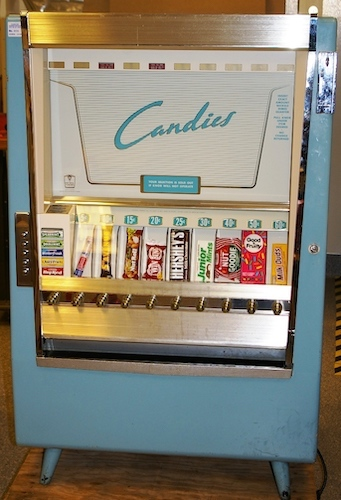
\includegraphics[scale=0.4]{CandiesVendingMachine1952}}

\end{figure}

{\tiny Source: Minnesota Historical Society, \href{https://creativecommons.org/licenses/by-sa/2.0}{CC BY-SA 2.0}}
\end{frame}

\begin{frame}[fragile]{The Vending Machine}
\begin{itemize}
\item Final project is a vending machine
\item Inputs: coins, buy
\item Display: price and current amount
\item Output: release can or error
\item Small challenge to multiplex the display
\item State machine with data path is the \emph{brain} of the VM
\item Will be guided step by step over several weeks
\end{itemize}
\end{frame}


\begin{frame}[fragile]{Combinational Circuit with Conditional Update}
\begin{itemize}
\item Value first needs to be wrapped into a \code{Wire}
\item Updates with the Chisel update operation \code{:=}
\item With \code{when} we can express a conditional update
\item The condition is an expression with a Boolean result
\item The resulting circuit is a multiplexer
\item The rule is that the last enabled assignment counts
\begin{itemize}
\item Here the order of statements has a meaning
\end{itemize}
\end{itemize}
\shortlist{../code/comb_wire2.txt}
\end{frame}

\begin{frame}[fragile]{Comparison}
\begin{itemize}
\item The usual operations
\begin{itemize}
\item Unusual equal and unequal operator symbols
\item To keep the original Sala operators usable for references
\end{itemize}
\item Operands are \code{UInt} and \code{SInt}
\item Operands can be \code{Bool} for equal and unequal
\item Result is \code{Bool}
\end{itemize}
\begin{chisel}
===, =/=
>, >=, <, <=
\end{chisel}
\end{frame}

\begin{frame}[fragile]{Boolean Logical Operations}
\begin{itemize}
\item Operands and result are \code{Bool}
\item Logical NOT, AND, and OR
\end{itemize}
\begin{chisel}
val notX = !x
val bothTrue = a && b
val orVal = x || y
\end{chisel}
\end{frame}

\begin{frame}[fragile]{The ``Else'' Branch}
\begin{itemize}
\item We can express a form of ``else''
\item Note the \code{.} in \code{.otherwise}
\end{itemize}
\shortlist{../code/comb_otherwise.txt}
\end{frame}



\begin{frame}[fragile]{A Chain of Conditions}
\begin{itemize}
\item To test for different conditions
\item Select with a priority order
\item The first that is true counts
\item The hardware is a chain of multiplexers
\end{itemize}
\begin{columns}
\column{0.5\textwidth}
\shortlist{../code/comb_elsewhen.txt}
\column{0.5\textwidth}
\begin{figure}
  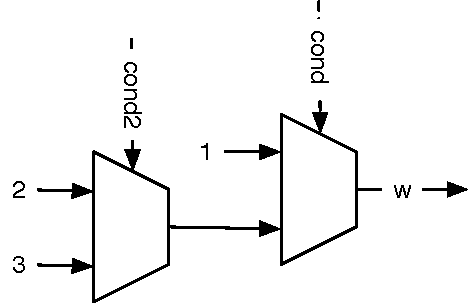
\includegraphics[scale=\scale]{../figures/mux-chain}
\end{figure}
\end{columns}
\end{frame}

\begin{frame}[fragile]{Default Assignment}
\begin{itemize}
\item Practical for complex expressions
\item Forgetting to assign a value on all conditions
\begin{itemize}
\item Would describe a latch
\item Runtime error in Chisel
\end{itemize}
\item Assign a default value is good practise
\end{itemize}
\shortlist{../code/comb_wiredefault.txt}
\end{frame}

\begin{frame}[fragile]{Logic Can Be Expressed as a Table}
\begin{itemize}
\item Sometimes more convenient 
\item Still combinational logic (gates)
\item Is converted to Boolean expressions
\item Let the synthesize tool do the conversion!
\item We use the \code{switch} statement
\end{itemize}
\shortlist{../code/encdec_dec.txt}
\end{frame}


\begin{frame}[fragile]{A Decoder}
\begin{figure}
  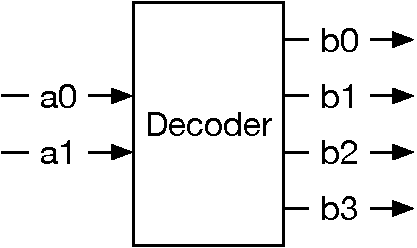
\includegraphics[scale=\scale]{../figures/decoder}
\end{figure}
\begin{itemize}
\item Converts a binary number of $n$ bits to an $m$-bit signal, where $m \leq 2^n$
\item The output is one-hot encoded (exactly one bit is one)
\item Building block for a $m$-way Mux
\item Used for address decoding in a computer system
\end{itemize}
\end{frame}

\begin{frame}[fragile]{Truth Table of a Decoder}
\begin{table}
  \begin{tabular}{rr}
    \toprule
    a & b \\
    \midrule
    00 & 0001 \\
    01 & 0010 \\
    10 & 0100 \\
    11 & 1000 \\
    \bottomrule 
  \end{tabular} 
\end{table}
\begin{itemize}
\item Does this look like the table we have seen?
\end{itemize}
\end{frame}

\begin{frame}[fragile]{Decoder in Chisel}
\begin{itemize}
\item Binary strings are a clearer representation
\end{itemize}
\shortlist{../code/encdec_decbin.txt}
\end{frame}

\begin{frame}[fragile]{An Encoder}
\begin{figure}
  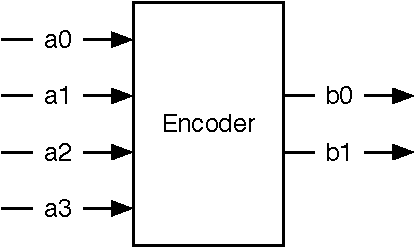
\includegraphics[scale=\scale]{../figures/encoder}
\end{figure}
\begin{itemize}
\item Converts one-hot encoded signal
\item To binary representation
\end{itemize}
\end{frame}

\begin{frame}[fragile]{Truth Table of an Encoder}
\begin{table}
  \begin{tabular}{rr}
    \toprule
    a & b \\
    \midrule
    0001 & 00 \\
    0010 & 01 \\
    0100 & 10 \\
    1000 & 11 \\
    ???? & ?? \\
    \bottomrule 
  \end{tabular} 
\end{table}
\begin{itemize}
\item Only defined for one-hot input
\end{itemize}
\end{frame}

\begin{frame}[fragile]{Encoder in Chisel}
\begin{itemize}
\item We cannot describe a function with undefined outputs
\item We use a default assignment of \code{"b00"}
\end{itemize}
\shortlist{../code/encdec_enc.txt}

\end{frame}

\begin{frame}[fragile]{Register (Again)}
\begin{itemize}
\item Sequential building blocks
\begin{itemize}
\item Contain a register
\item Plus combinational circuits
\end{itemize}
\end{itemize}
\begin{figure}
  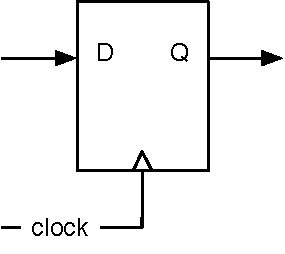
\includegraphics[scale=\scale]{../figures/register}
\end{figure}
\shortlist{../code/sequ_reg.txt}
\end{frame}



\begin{frame}[fragile]{Register in Two Steps}
\shortlist{../code/sequ_reg2.txt}
\end{frame}

\begin{frame}[fragile]{Register With Reset}
\begin{figure}
  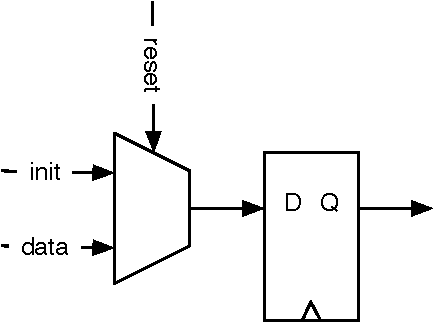
\includegraphics[scale=\scale]{../figures/register-reset}
\end{figure}
\shortlist{../code/sequ_reg_init.txt}
\end{frame}

\begin{frame}[fragile]{Timing Diagram of the Register with Reset}
\begin{figure}
  \includegraphics[scale=1]{../figures/reg_wave}
\end{figure}
\begin{itemize}
\item Also called waveform diagram
\item Logic function over time
\item Can be used to describe a circuit function
\item Useful for debugging
\end{itemize}
\end{frame}

\begin{frame}[fragile]{Register with Enable}
\begin{figure}
  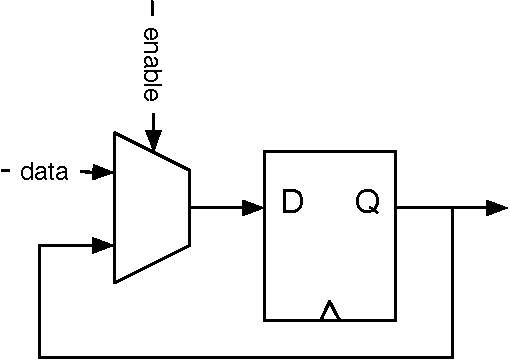
\includegraphics[scale=\scale]{../figures/register-enable}
\end{figure}
\begin{itemize}
\item Only when \code{enable} true is a value is stored
\end{itemize}
\shortlist{../code/sequ_reg_ena.txt}

\end{frame}

\begin{frame}[fragile]{Timing Diagram for an Enable Register}
\begin{figure}
  \includegraphics[scale=1]{../figures/reg_en_wave}
\end{figure}
\end{frame}

\begin{frame}[fragile]{More on Register}
\begin{itemize}
\item We can combine initialization and enable
\end{itemize}
\shortlist{../code/sequ_reg_init_ena.txt}
\begin{itemize}
\item A register can also be part of an expression
\item What does the following circuit do?
\end{itemize}
\shortlist{../code/sequ_reg_rising.txt}
\end{frame}


\begin{frame}[fragile]{Combine a Register with an Adder}
\begin{figure}
  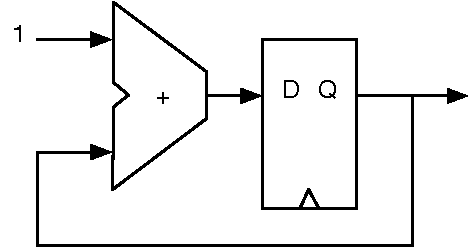
\includegraphics[scale=\scale]{../figures/counter}
\end{figure}
\begin{itemize}
\item Is a free running counter
\item 0, 1, ... 14, 15, 0, 1, ...
\end{itemize}
\shortlist{../code/sequ_free_counter.txt}
\end{frame}


\begin{frame}[fragile]{A Counter}
\shortlist{../code/counter.txt}
\begin{itemize}
\item This counter counts from 0 to 9
\item And starts from 0 again after reaching 9
\begin{itemize}
\item Starting from 0 is common in computer engineering
\end{itemize}
\item A counter is the hardware version of a \emph{for loop}
\item Often needed
\item Can you draw the schematic?
\end{itemize}
\end{frame}

\begin{frame}[fragile]{Counting Events}
\begin{figure}
  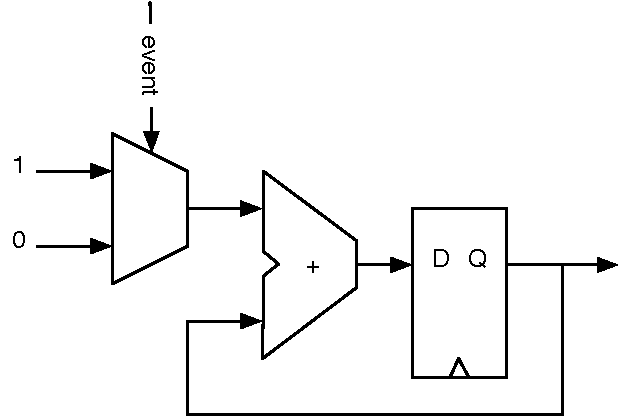
\includegraphics[scale=\scale]{../figures/event-counter}
\end{figure}
\begin{itemize}
\item Is the schematics and the code the same?
\end{itemize}
\shortlist{../code/sequ_event_counter.txt}
\end{frame}


\begin{frame}[fragile]{Structure With Bundles}
\begin{itemize}
\item A \code{Bundle} to groups signals
\item Can be different types
\item Defined by a class that extends \code{Bundle}
\item List the fields as \code{val}s within the block
\item Like a C struct or VHDL record
\end{itemize}
\shortlist{../code/bundle.txt}
\end{frame}

\begin{frame}[fragile]{Using a Bundle}
\begin{itemize}
\item Create it with \code{new}
\item Wrap it into a \code{Wire}
\item Field access with \emph{dot} notation
\end{itemize}
\shortlist{../code/bundle_use.txt}
\end{frame}

\begin{frame}[fragile]{A Collection of Signals with \code{Vec}}
\begin{itemize}
\item Chisel \code{Vec} is a collection of signals of the same type
\item The collection can be accessed by an index
\item Similar to an array in other languages
\end{itemize}
\shortlist{../code/vec.txt}
\end{frame}

\begin{frame}[fragile]{Using a \code{Vec}}
\shortlist{../code/vec_access.txt}
\begin{itemize}
\item Reading from an \code{Vec} is a multplexer
\item We can put a \code{Vec} into a \code{Reg}
\end{itemize}
\shortlist{../code/reg_file.txt}
\noindent An element of that register file is accessed with an index and used as a normal register.

\shortlist{../code/reg_file_access.txt}
\end{frame}


\begin{frame}[fragile]{Mixing Vecs and Bundles}
\begin{itemize}
\item We can freely mix bundles and vectors
\item When creating a vector with a bundle
type, we need to pass a prototype for the vector fields. Using our
\code{Channel}, which we defined above, we can create a vector of channels with:
\end{itemize}
\shortlist{../code/vec_bundle.txt}
\begin{itemize}
\item A bundle may as well contain a vector
\end{itemize}
\shortlist{../code/bundle_vec.txt}
\end{frame}

\begin{frame}[fragile]{Power User II}
\begin{itemize}
\item xxx
 * Talk about tools
   * see chapter 3 in pragmatic programmer
   * Tools amplify your talent. The better your tools, and the better you know how to use them, the more productive you can be.
   * Talk about google, man pages, or even plain --help
 * Use (and write) tools
 * link is missing: use simple bash scripts or Makefiles to remember commands (show examples)


 * Do power user in week 4
 * Have some slides, but mostly show demo
 * link to Linux intro
 * Use the Windows VM
 * open a powershell terminal
 * do a mkdir
 * do ls and cd
 * open browser to repo and copy string
 * do a git clone
 * cd and ls, maybe a cat
 * setup IntelliJ
 * run one exercise
 * switch to Mac and change minor thing
 * Do git commit/push
 * do a git pull in Windows, show in IntelliJ README.md
 * On Mac go to GitHub page
 * Do a change
 * On Windows do a git pull in IntelliJ
 * Say to take it easy, you do not need to do this, but it will help you to become a better engineer ;-)
\item \url{https://www.oreilly.com/learning/ten-steps-to-linux-survival}

\end{itemize}
\end{frame}

\begin{frame}[fragile]{Power User II}
\begin{itemize}
\item Every craftsmen starts with good-quality tools
\item ``Tools amplify your talent''\footnote{The Pragmatic Programmer: From Journeyman to Master, by Andrew Hunt and David Thomas}
\begin{itemize}
\item The better your tools, the more productive you are
\item The better you know them, the more productive you are
\end{itemize}
\item IDEs (Eclipse, InelliJ) are nice, I love them too
\item But we shall go beyond it
\item
\item
\item
\end{itemize}
\end{frame}

\begin{frame}[fragile]{XXX}
\begin{itemize}
\item
\item
\item
\end{itemize}
\end{frame}

\begin{frame}[fragile]{XXX}
\begin{itemize}
\item
\item
\item
\end{itemize}
\end{frame}


\begin{frame}[fragile]{XXX}
\begin{itemize}
\item xxx
\begin{itemize}
\item
\end{itemize}
\item
\item
\item
\item
\item
\end{itemize}
\end{frame}


\begin{frame}[fragile]{Verilog Generation}
\begin{itemize}
\item TODO: show individual snippets
\item on @[Hello.scala 17:23]
\begin{itemize}
\item
\end{itemize}
\item about pin names, e.g., \code{io\_led}
\item
\item
\item
\item
\end{itemize}
\begin{verbatim}
module Hello(
  input   clock,
  input   reset,
  output  io_led
);
  reg [31:0] cntReg; // @[Hello.scala 17:23]
  reg [31:0] _RAND_0;
  reg  blkReg; // @[Hello.scala 18:23]
  reg [31:0] _RAND_1;
  wire [31:0] _T_1; // @[Hello.scala 20:20]
  wire  _T_2; // @[Hello.scala 21:15]
  wire  _T_3; // @[Hello.scala 23:15]
  assign _T_1 = cntReg + 32'h1; // @[Hello.scala 20:20]
  assign _T_2 = cntReg == 32'h2faf07f; // @[Hello.scala 21:15]
  assign _T_3 = ~ blkReg; // @[Hello.scala 23:15]
  assign io_led = blkReg; // @[Hello.scala 25:10]
`ifdef RANDOMIZE_GARBAGE_ASSIGN
`define RANDOMIZE
`endif
`ifdef RANDOMIZE_INVALID_ASSIGN
`define RANDOMIZE
`endif
`ifdef RANDOMIZE_REG_INIT
`define RANDOMIZE
`endif
`ifdef RANDOMIZE_MEM_INIT
`define RANDOMIZE
`endif
`ifndef RANDOM
`define RANDOM $random
`endif
`ifdef RANDOMIZE_MEM_INIT
  integer initvar;
`endif
`ifndef SYNTHESIS
initial begin
  `ifdef RANDOMIZE
    `ifdef INIT_RANDOM
      `INIT_RANDOM
    `endif
    `ifndef VERILATOR
      `ifdef RANDOMIZE_DELAY
        #`RANDOMIZE_DELAY begin end
      `else
        #0.002 begin end
      `endif
    `endif
  `ifdef RANDOMIZE_REG_INIT
  _RAND_0 = {1{`RANDOM}};
  cntReg = _RAND_0[31:0];
  `endif // RANDOMIZE_REG_INIT
  `ifdef RANDOMIZE_REG_INIT
  _RAND_1 = {1{`RANDOM}};
  blkReg = _RAND_1[0:0];
  `endif // RANDOMIZE_REG_INIT
  `endif // RANDOMIZE
end // initial
`endif // SYNTHESIS
  always @(posedge clock) begin
    if (reset) begin
      cntReg <= 32'h0;
    end else if (_T_2) begin
      cntReg <= 32'h0;
    end else begin
      cntReg <= _T_1;
    end
    if (reset) begin
      blkReg <= 1'h0;
    end else if (_T_2) begin
      blkReg <= _T_3;
    end
  end
endmodule

\end{verbatim}
\end{frame}

\begin{frame}[fragile]{File Organization in Scala/Chisel}
\begin{itemize}
\item A Scala file can contain several classes (and objects)
\item For large classes use one file per class with the class name
\item Scala has packages, like Java
\item Use folders with the package names for file organization
\item \code{sbt} looks into current folder and \code{src/main/scala/}
\item Tests shall be in \code{src/test/scala/}
\end{itemize}
\end{frame}

\begin{frame}[fragile]{File Organization in Scala/Chisel}
\dirtree{%
.1 project.
.2 src.
.3 main.
.4 scala.
.5 package.
.6 sub-package.
.3 test.
.4 scala.
.5 package.
.2 target.
.2 generated.
}
\end{frame}

\begin{frame}[fragile]{XXX}
\begin{itemize}
\item xxx
\begin{itemize}
\item
\end{itemize}
\item
\item
\item
\item
\item
\end{itemize}
\end{frame}


\begin{frame}[fragile]{XXX}
\begin{itemize}
\item xxx
\begin{itemize}
\item
\end{itemize}
\item
\item
\item
\item
\item
\end{itemize}
\end{frame}

\begin{frame}[fragile]{Common Acronyms}
\begin{description}
\item [ADC] analog-to-digital converter
\item [ALU] arithmetic and logic unit
\item [ASIC] application-specific integrated circuit
\item [Chisel] constructing hardware in a Scala embedded language
\item [CISC] complex instruction set computer
\item [CRC] cyclic redundancy check
\item [DFF] D flip-flop, data flip-flop
\item [DMA] direct memory access
\item [DRAM] dynamic random access memory
\item [FF] flip-flop
\item [FIFO] first-in, first-out
\item [FPGA] field-programmable gate array
\item [HDL] hardware description language
\item [HLS] high-level synthesis
\item [IC] instruction count
\item [IDE] integrated development environment
\item [IO] input/output
\end{description}
\end{frame}

\begin{frame}[fragile]{Common Acronyms II}
\begin{description}
\item [ISA] instruction set architecture
\item [JDK] Java development kit
\item [JIT] just-Iin-time
\item [JVM] Java virtual machine
\item [LC] logic cell
\item [LRU] least-recently used
\item [MMIO] memory-mapped IO
\item [MUX] multiplexer
\item [OO] object oriented
\item [RISC] reduced instruction set computer
\item [SDRAM] synchronous DRAM
\item [SRAM] static random access memory
\item [TOS] top-of stack
\item [UART] universal asynchronous receiver/transmitter
\item [VHDL] VHSIC hardware description language
\item [VHSIC] very high speed integrated circuit
\end{description}
\end{frame}

\begin{frame}[fragile]{Chisel VHDL Comparison}
\begin{columns}
\column{0.5\textwidth}
\begin{chisel}
class DecodeExecute extends Bundle {
  val rs1 = UInt(32.W)
  val rs2 = UInt(32.W)
  val immVal = UInt(32.W)
  val aluOp = new AluOp()
}
\end{chisel}
\column{0.5\textwidth}
\begin{verbatim}
VHDL code here
\end{verbatim}
\end{columns}
Also show latch and and using a button as clock
\end{frame}

\begin{frame}[fragile]{Lab Today}
\begin{itemize}
\item Combinational circuits in Chisel
\item \href{https://github.com/schoeberl/chisel-lab/tree/master/lab4}{Lab 4 Page}
\item You need to download again, as I have updated the lab
\begin{itemize}
\item Or learn to use git and do a  \code{git pull} ;-)
\end{itemize}
\item Each exercise contains a test, which initially fails
\item \code{sbt test} runs them all
\begin{itemize}
\item To just run a single test, run e.g.,\\
\code{sbt "testOnly MajorityPrinter"}
\end{itemize}
When all test succeed your are done ;-)
\item Components contain a comment where you shall add your implementation
\item The initial majority example has an optional implementation in an FPGA
\end{itemize}
\end{frame}

\begin{frame}[fragile]{Lab Time}
\begin{itemize}
\item xxx
\item
\item
\item
\end{itemize}
\end{frame}

\begin{frame}[fragile]{Summary}
\begin{itemize}
\item xxx
\item
\item
\item
\end{itemize}
\end{frame}

\begin{frame}[fragile]{XXX}
\begin{itemize}
\item xxx
\item
\item
\item
\end{itemize}
\end{frame}

\begin{frame}[fragile]{Functional Abstraction}
\begin{chisel}
  def addSub(add: Bool, a: UInt, b: UInt) =
    Mux(add, a+b, a-b)

  val res = addSub(cond, a, b)
  
  def rising(d: Bool) = d && !RegNext(d)
\end{chisel}
\begin{itemize}
\item Functions for repeated pieces of logic
\item May contain state
\item Functions may return \emph{hardware}
\end{itemize}
\end{frame}


\begin{frame}[fragile]{Bundles}
\begin{chisel}
class DecodeExecute extends Bundle {
  val rs1 = UInt(32.W)
  val rs2 = UInt(32.W)
  val immVal = UInt(32.W)
  val aluOp = new AluOp()
}
\end{chisel}
\begin{itemize}
\item Collection of values in named fields 
\item Like struct or record
\end{itemize}
\end{frame}

\begin{frame}[fragile]{Vectors}
\begin{chisel}
val myVec = Vec(3, SInt(10.W))

myVec(0) := -3.S
val y = myVec(2)
\end{chisel}
\begin{itemize}
\item Indexable vector of elements
\item Bundles and Vecs can be arbitrarely nested
\end{itemize}
\end{frame}





\begin{frame}[fragile]{IO Ports}
\begin{chisel}
class Channel extends Bundle {
  val data = Input(UInt(8.W))
  val ready = Output(Bool())
  val valid = Input(Bool())
}
\end{chisel}
\begin{itemize}
\item Ports are Bundles with directions
\item Direction can also be assigned at instantiation:
\end{itemize}
\begin{chisel}
class ExecuteIO extends Bundle {
  val dec = Input(new DecodeExecute())
  val mem = Output(new ExecuteMemory())
}
\end{chisel}
\end{frame}

\begin{frame}[fragile]{Modules}
\begin{chisel}
class Adder extends Module {
  val io = IO(new Bundle {
    val a = Input(UInt(4.W))
    val b = Input(UInt(4.W))
    val result = Output(UInt(4.W))
  })

  val addVal = io.a + io.b
  io.result := addVal
}
\end{chisel}
\begin{itemize}
\item Organization of components
\item IO ports defined as a Bundle named \code{io} and wrapped into an \code{IO()}
\item Created (instantiated) with:
\end{itemize}
\begin{chisel}
val adder = Module(new Adder())
\end{chisel}
\end{frame}

\begin{frame}[fragile]{Connections}
\begin{itemize}
\item Simple connections just with assignments, e.g.,
\begin{chisel}
  adder.io.a := ina
  adder.io.b := inb
\end{chisel}
\item Automatic bulk connections between components
\begin{chisel}
  dec.io <> exe.io
  mem.io <> exe.io
\end{chisel}
\end{itemize}
\end{frame}

\begin{frame}[fragile]{Ports}
\begin{itemize}
\item Ports used to connect modules
\item Ports are bundles with directions
\end{itemize}
\begin{chisel}
class AluIO extends Bundle {
  val function = Input(UInt(2.W))
  val inputA = Input(UInt(4.W))
  val inputB = Input(UInt(4.W))
  val result = Output(UInt(4.W))
}
\end{chisel}
\end{frame}

\begin{frame}[fragile]{Port Directions}
\begin{itemize}
\item Can be assigned at instantiation
\end{itemize}
\begin{chisel}
class ExecuteIO extends Bundle {
  val dec = Input(new DecodeExecute())
  val mem = Output(new ExecuteMemory())
}
\end{chisel}
\begin{chisel}
\end{chisel}
\end{frame}

\begin{frame}[fragile]{Port Directions}
\begin{itemize}
\item Can be reversed with the \code{Flipped}
\item Convenient to have one bundle definition working as source
and destination used between two modules
\end{itemize}
\begin{chisel}
class Channel extends Bundle {
  val data = Input(UInt(32.W))
  val ready = Output(Bool())
  val valid = Input(Bool())
}

class ChannelUsage extends Bundle {
  val input = new Channel()
  val output = Flipped(new Channel())
}
\end{chisel}
\end{frame}

\begin{frame}[fragile]{Modules}
\begin{itemize}
\item Modules are used to organize the circuit
\item Similar to VHDL components (entity/architecture)
\item A class that inherits from \code{Module}
\item Circuit description in the constructor
\item Interface (port) is a \code{Bundle}, wrapped into an \code{IO()}, and stored in the field \code{io}
\end{itemize}
\begin{chisel}
class Adder extends Module {
  val io = IO(new Bundle {
    val a = Input(UInt(4.W))
    val b = Input(UInt(4.W))
    val result = Output(UInt(4.W))
  })

  val addVal = io.a + io.b
  io.result := addVal
}
\end{chisel}
\end{frame}

\begin{frame}[fragile]{Module Usage}
\begin{itemize}
\item Create with \code{new} and wrap into a \code{Module()}
\item Interface port via the \code{io} field
\item Note the assignment operator \code{:=} on \code{io} fields
\end{itemize}
\begin{chisel}
  val adder = Module(new Adder())
  adder.io.a := ina
  adder.io.b := inb
  val result = adder.io.result
\end{chisel}
\end{frame}


\begin{frame}[fragile]{Chisel and Scala}
\begin{itemize}
\item Chisel is a library written in Scala
\begin{itemize}
\item Import the library with \code{import chisel3.\_}
\end{itemize}
\item Chisel code is Scala code
\item When it is run is \emph{generates} hardware
\begin{itemize}
\item Verilog for synthesize
\item Scala netlist for simulation (testing)
\end{itemize}
\item Chisel is an embedded domain specific language
\item Two languages in one can be a little bit confusing
\end{itemize}
\end{frame}

\begin{frame}[fragile]{Scala}
\begin{itemize}
\item Is object oriented
\item Is functional
\item Strongly typed with very good type inference
\item Runs on the Java virtual machine
\item Can call Java libraries
\item Consider it as Java++
\begin{itemize}
\item Can almost be written like Java
\item With a more lightweight syntax
\item Scala for Java Refugees is a nice tutorial
\item \url{http://www.codecommit.com/blog/scala/roundup-scala-for-java-refugees}
\end{itemize}
\end{itemize}
\end{frame}

\begin{frame}[fragile]{Scala Hello World}
\begin{chisel}
object HelloWorld extends App {
  println("Hello, World!")
}
\end{chisel}
\begin{itemize}
\item Compile with \code{scalac} and run with \code{scala}
\item You can even use Scala as scripting language
\item Show both
\end{itemize}
\end{frame}



\begin{frame}[fragile]{Generic Components}
\begin{chisel}
val c = Mux(cond, a, b)
\end{chisel}
\begin{itemize}
\item This is a multiplexer
\item Input can be any type
\end{itemize}
\end{frame}

\begin{frame}[fragile]{Testing}
\begin{chisel}
class CounterTester(c: Counter) extends PeekPokeTester(c) {
  for (i <- 0 until 5) {
    println(i.toString + ": " + peek(c.io.out).toString())
    step(1)
  }
}
\end{chisel}
\begin{itemize}
\item Within Chisel with a tester (= Scala program)
\item May include waveform generation
\item peek and poke to read and set values
\begin{itemize}
\item Remember the BASIC days ;-)
\end{itemize}
\item printf in simulation on rising edge
\begin{chisel}
printf("Counting %x\n", r1)
\end{chisel}
\end{itemize}
\end{frame}

\begin{frame}[fragile]{Component Generation}
\begin{chisel}
val cores = new Array[Module](32)

for (j <- 0 until 32)
  cores(j) = Module(new CPU())
\end{chisel}
\begin{itemize}
\item Use Scala array to collect components
\item Generation with a Scala loop
\end{itemize}
\end{frame}

\begin{frame}[fragile]{Conditional Component Generation}
\begin{chisel}
val icache =
  if (TYPE == METHOD)
    Module(new MCache())
  else if (TYPE == LINE)
    Module(new ICache())
  else
    ChiselError.error("Unsupported Type")
\end{chisel}
\begin{itemize}
\item Use Scala if/else for conditional component types
\item Code example from Patmos
\item We parse an XML file for the configuration
\end{itemize}
\end{frame}

\begin{frame}[fragile]{Logic Generation}
\begin{itemize}
\item Read a file into a table
\begin{itemize}
\item E.g., to read in ROM content for a processor
\end{itemize}
\item Generate a truth table algorithmically
\begin{itemize}
\item E.g., generate binary to BCD translation
\end{itemize}
\item Use the full power of Scala
\end{itemize}
\begin{chisel}
val byteArray = Files.readAllBytes(Paths.get(fileName))
val arr = new Array[Bits](byteArray.length)
for (i <- 0 until byteArray.length) {
  arr(i) = Bits(byteArray(i), 8)
}
val rom = Vec[Bits](arr)
\end{chisel}
\end{frame}
%%%%%%%%%%%%%%%%%
%\begin{frame}[fragile]{zzz}
%\begin{chisel}
%code
%\end{chisel}
%\begin{itemize}
%\item xxx
%\item xxx
%\item xxx
%\end{itemize}
%\end{frame}
%
%\begin{frame}[fragile]{yyy}
%\begin{itemize}
%\item xxx
%\item xxx
%\item xxx
%\item xxx
%\item xxx
%\end{itemize}
%\end{frame}
%%%%%%%%%%%%%%%%%

\begin{frame}[fragile]{Scala Values and Variables}
\begin{chisel}
// A value is a constant
val i = 0
// No new assignment; this will not compile
i = 3

// A variable can change the value
var v = "Hello"
v = "Hello World"

// Type usually inferred, but can be declared
var s: String = "abc"
\end{chisel}
\end{frame}

\begin{frame}[fragile]{Simple Loops}
\begin{chisel}
// Loops from 0 to 9
// Automatically creates loop value i
for (i <- 0 until 10) {
  println(i)
}
\end{chisel}
\end{frame}

\begin{frame}[fragile]{Conditions}
\begin{chisel}
for (i <- 0 until 10) {
  if (i%2 == 0) {
    println(i + " is even")
  } else {
    println(i + " is odd")
  }
}
\end{chisel}
\end{frame}

\begin{frame}[fragile]{Scala Arrays and Lists}
\begin{chisel}
// An integer array with 10 elements
val numbers = new Array[Integer](10)
for (i <- 0 until numbers.length) {
  numbers(i) = i*10
}
println(numbers(9))


// List of integers
val list = List(1, 2, 3)
println(list)
// Different form of list construction
val listenum = 'a' :: 'b' :: 'c' :: Nil
println(listenum)
\end{chisel}
\end{frame}


\begin{frame}[fragile]{Scala Classes}
\begin{chisel}
// A simple class
class Example {
  // A field, initialized in the constructor
  var n = 0
  
  // A setter method
  def set(v: Integer) = {
    n = v
  }
  
  // Another method
  def print() = {
    println(n)
  }
}
\end{chisel}
\end{frame}

\begin{frame}[fragile]{Scala (Singleton) Object}
\begin{chisel}
object Example {}
\end{chisel}
\begin{itemize}
\item For \emph{static} fields and methods
\begin{itemize}
\item Scala has no static fields or methods like Java
\end{itemize}
\item Needed for \code{main}
\item Useful for helper functions
\end{itemize}
\end{frame}

\begin{frame}[fragile]{Singleton Object for the \code{main}}
\begin{chisel}
// A singleton object
object Example {
  
  // The start of a Scala program
  def main(args: Array[String]): Unit = {
    
    val e = new Example()
    e.print()
    e.set(42)
    e.print()
  }
}
\end{chisel}
\begin{itemize}
\item Compile and run it with sbt (or within Eclipse/IntelliJ):
\end{itemize}
\begin{chisel}
sbt "runMain Example"
\end{chisel}
\end{frame}

\begin{frame}[fragile]{Scala Build Tool (sbt)}
\begin{itemize}
\item Downloads Scala compiler if needed
\item Downloads dependent libraries (e.g., Chisel)
\item Compiles Scala programs
\item Executes Scala programs
\item Does a lot of magic, maybe too much
\item Compile and run with:
\end{itemize}
\begin{chisel}
sbt "runMain simple.Example"
\end{chisel}
\begin{itemize}
\item Or even just:
\end{itemize}
\begin{chisel}
sbt run
\end{chisel}
\end{frame}

\begin{frame}[fragile]{Build Configuration}
\begin{itemize}
\item Defines needed Scala version
\item Library dependencies
\item File name: \code{build.sbt}
\end{itemize}
\begin{chisel}
scalaVersion := "2.11.7"

resolvers ++= Seq(
  Resolver.sonatypeRepo("snapshots"),
  Resolver.sonatypeRepo("releases")
)

libraryDependencies += "edu.berkeley.cs" %% "chisel3" % "3.1.2"
libraryDependencies += "edu.berkeley.cs" %% "chisel-iotesters" % "1.2.2"
\end{chisel}
\end{frame}


\begin{frame}[fragile]{What is a Minimal Chisel Project?}
\begin{itemize}
\item Scala class (e.g., \code{Hello.scala})
\item Build info in \code{build.sbt} for \code{sbt}:
\end{itemize}
\begin{chisel}
scalaVersion := "2.11.7"

libraryDependencies += "edu.berkeley.cs" %% "chisel3" % "3.1.2"
\end{chisel}
\begin{itemize}
\item Run the process manually (look into the Makefile)
\end{itemize}
\end{frame}

\begin{frame}[fragile]{File Organization in Scala/Chisel}
\begin{itemize}
\item A Scala file can contain several classes (and objects)
\item For large classes use one file per class with the class name
\item Scala has packages, like Java
\item Use folders with the package names for file organization
\item \code{sbt} looks into current folder and \code{src/main/scala/}
\item Tests shall be in \code{src/test/scala/}
\end{itemize}
\end{frame}

\begin{frame}[fragile]{File Organization in Scala/Chisel}
\dirtree{%
.1 project.
.2 src.
.3 main.
.4 scala.
.5 package.
.6 sub-package.
.3 test.
.4 scala.
.5 package.
.2 target.
.2 generated.
}
\end{frame}

\begin{frame}[fragile]{Chisel Main}

\begin{itemize}
\item Create one top-level Module
\item Invoke the Chisel driver from the Scala \code{main} (or App)
\item Pass some parameters and the top module
\item Following code generates Verilog code
\end{itemize}
\begin{chisel}
object Hello extends App {
  chisel3.Driver.execute(Array[String](), () => new Hello())
}
\end{chisel}
\end{frame}

\begin{frame}[fragile]{Chisel Main for Testing}
\begin{itemize}
\item Tests can be written in Scala/Chisel
\item Tester and device under test (DUT) are two processes
\item Invoke \code{execute} with some parameters, the DUT, and a tester
\end{itemize}
\begin{chisel}
object CounterTester extends App {

  iotesters.Driver.execute(Array[String](), () => new Counter(2)) {
    c => new CounterTester(c)
  }
}
\end{chisel}
\end{frame}

\begin{frame}[fragile]{A Chisel Tester}
\begin{itemize}
\item Extends class \code{PeekPokeTester}
\item Has the DUT as parameter
\item Testing code can use all features of Scala
\end{itemize}
\begin{chisel}
class CounterTester(dut: Counter) extends PeekPokeTester(dut) {

  // Here comes the Chisel/Scala code
  // for the testing
}
\end{chisel}
\end{frame}

\begin{frame}[fragile]{Testing}
\begin{itemize}
\item Set input values with \code{poke}
\item Advance the simulation with \code{step}
\item Read the output values with \code{peek}
\item Compare the values with \code{expect}
\end{itemize}
\end{frame}

\begin{frame}[fragile]{Testing Example}
\begin{chisel}
// Set input values
poke(dut.io.a, 3)
poke(dut.io.b, 4)
// Execute one iteration
step(1)
// Print the result
val res = peek(dut.io.result)
println(res)

// Or compare against expected value
expect(dut.io.result, 7)
\end{chisel}
\end{frame}

\begin{frame}[fragile]{A Tiny ALU: IO Connection}
\begin{chisel}
class Alu extends Module {
  val io = IO(new Bundle {
    val fn = Input(UInt(2.W))
    val a = Input(UInt(4.W))
    val b = Input(UInt(4.W))
    val result = Output(UInt(4.W))
  })

  // Use shorter variable names
  val fn = io.fn
  val a = io.a
  val b = io.b
\end{chisel}
\end{frame}

\begin{frame}[fragile]{A Tiny ALU: The Function}
\begin{chisel}
  val result = Wire(UInt(4.W))
  // some default value is needed
  result := 0.U

  // The ALU selection
  switch(fn) {
    is(0.U) { result := a + b }
    is(1.U) { result := a - b }
    is(2.U) { result := a | b }
    is(3.U) { result := a & b }
  }

  // Output on the LEDs
  io.result := result
}
\end{chisel}
\end{frame}

\begin{frame}[fragile]{Testing the ALU}
\begin{itemize}
\item Compute the expected result in Scala
\end{itemize}
\begin{chisel}
  // This is exhaustive testing,
  // which usually is impossible
  for (a <- 0 to 15) {
    for (b <- 0 to 15) {
      for (op <- 0 to 3) {
        val result =
          op match {
            case 0 => a + b
            case 1 => a - b
            case 2 => a | b
            case 3 => a & b
          }
        val resMask = result & 0x0f
\end{chisel}

\end{frame}

\begin{frame}[fragile]{Testing the ALU}
\begin{itemize}
\item Compare the Scala computed result with the hardware result
\end{itemize}
\begin{chisel}
        poke(dut.io.fn, op)
        poke(dut.io.a, a)
        poke(dut.io.b, b)
        step(1)
        expect(dut.io.result, resMask)
      }
    }
  }
\end{chisel}
\end{frame}

\begin{frame}[fragile]{Generating Wave Forms}
\begin{itemize}
\item Additional parameters: \code{"--generate-vcd-output", "on"}
\item IO signals and registers are dumped
\item Option \code{--debug} puts all wires into the dump
\item Generates a .vcd file
\item Viewing with gtkwave or ModelSim
\item See the example with \code{make fifo}
\begin{itemize}
\item Show it
\end{itemize}
\item BubbleFifo contains also longer testing code
\end{itemize}
\end{frame}

\begin{frame}[fragile]{Functions}
\begin{itemize}
\item Circuits can be encapsulated in functions
\item Each \emph{function call} generates hardware
\item Simple functions can be a single line
\end{itemize}
\begin{chisel}
  def adder(v1: UInt, v2: UInt) = v1 + v2
  
  val add1 = adder(a, b)
  val add2 = adder(c, d)
\end{chisel}
\end{frame}

\begin{frame}[fragile]{More Function Examples}
\begin{itemize}
\item Functions can also contain registers
\end{itemize}
\begin{chisel}
  def addSub(add: Bool, a: UInt, b: UInt) =
    Mux(add, a + b, a - b)

  val res = addSub(cond, a, b)

  def rising(d: Bool) = d && !RegNext(d)

  val edge = rising(cond)
\end{chisel}
\end{frame}

\begin{frame}[fragile]{The Counter as a Function}
\begin{itemize}
\item Longer functions in curly brackets
\item Last value is the return value
\end{itemize}
\begin{chisel}
def counter(n: UInt) = {
  
  val cntReg = RegInit(0.U(8.W))
  
  cntReg := cntReg + 1.U
  when(cntReg === n) {
    cntReg := 0.U
  }
  cntReg
}

val counter100 = counter(100.U)
\end{chisel}
\end{frame}


\begin{frame}[fragile]{Functions}
\begin{itemize}
\item Example from Patmos execute stage
\end{itemize}
\begin{chisel}
def alu(func: Bits, op1: UInt, op2: UInt): Bits = {
  val result = UInt(width = DATA_WIDTH)
  // some more lines...
  switch(func) {
    is(FUNC_ADD) { result := sum }
    is(FUNC_SUB) { result := op1 - op2 }
    is(FUNC_XOR) { result := (op1 ^ op2).toUInt }
    // some more lines
  }
  result
}
\end{chisel}
\end{frame}

\begin{frame}[fragile]{Scala List for Enumeration}
\begin{chisel}
  val empty :: full :: Nil = Enum(2)
\end{chisel}
\begin{itemize}
\item Can be used in wires and registers
\item Symbols for a state machine
\end{itemize}
\end{frame}

\begin{frame}[fragile]{Finite State Machine}
\begin{chisel}
  val empty :: full :: Nil = Enum(2)
  val stateReg = RegInit(empty)
  val dataReg = RegInit(0.U(size.W))

  when(stateReg === empty) {
    when(io.enq.write) {
      stateReg := full
      dataReg := io.enq.din
    }
  }.elsewhen(stateReg === full) {
    when(io.deq.read) {
      stateReg := empty
    }
  }
\end{chisel}
\begin{itemize}
\item A simple buffer for a bubble FIFO
\end{itemize}
\end{frame}

\begin{frame}[fragile]{Parameterization}
\begin{chisel}
class ParamChannel(n: Int) extends Bundle {
  val data = Input(UInt(n.W))
  val ready = Output(Bool())
  val valid = Input(Bool())
}

val ch32 = new ParamChannel(32)
\end{chisel}
\begin{itemize}
\item Bundles and modules can be parametrized
\item Pass a parameter in the constructor
\end{itemize}

\end{frame}
\begin{frame}[fragile]{A Module with a Parameter}
\begin{chisel}
class ParamAdder(n: Int) extends Module {
  val io = IO(new Bundle {
    val a = Input(UInt(n.W))
    val b = Input(UInt(n.W))
    val result = Output(UInt(n.W))
  })

  val addVal = io.a + io.b
  io.result := addVal
}

val add8 = Module(new ParamAdder(8))
\end{chisel}
\begin{itemize}
\item Parameter can also be a Chisel type
\item Can also be a generic type:
\item \code{class Mod[T <: Bits](param: T) extends...}
\end{itemize}
\end{frame}

\begin{frame}[fragile]{Scala \code{for} Loop for Circuit Generation}
\begin{chisel}
val shiftReg = RegInit(0.U(8.W))

shiftReg(0) := inVal

for (i <- 1 until 8) {
  shiftReg(i) := shiftReg(i-1)
}
\end{chisel}
\begin{itemize}
\item \code{for} is Scala
\item This loop generates several connections
\item The connections are parallel hardware
\end{itemize}
\end{frame}

\begin{frame}[fragile]{Conditional Circuit Generation}
\begin{chisel}
class Base extends Module { val io = new Bundle() }
class VariantA extends Base { }
class VariantB extends Base { }

val m = if (useA) Module(new VariantA())
        else Module(new VariantB())
\end{chisel}
\begin{itemize}
\item \code{if} and \code{else} is Scala
\item \code{if} is an expression that returns a value
\begin{itemize}
\item Like ``\code{cond ? a : b;}'' in C and Java
\end{itemize}
\item This is not a hardware multiplexer
\item Decides which module to generate
\item Could even read an XML file for the configuration
\end{itemize}
\end{frame}

%\begin{frame}[fragile]{Chisel has a Multiplexer}
\begin{figure}
  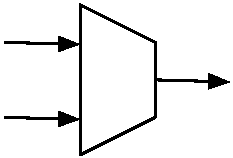
\includegraphics[scale=\scale]{../figures/mux}
\end{figure}
\shortlist{../code/mux.txt}
\begin{itemize}
\item So what?
\item Wait... What type is \code{a} and \code{b}?
\begin{itemize}
\item Can be any Chisel type!
\end{itemize}
\end{itemize}
\end{frame}

\begin{frame}[fragile]{Chisel has a Multiplexer}
\begin{figure}
  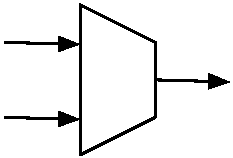
\includegraphics[scale=\scale]{../figures/mux}
\end{figure}
\shortlist{../code/mux.txt}
\begin{itemize}
\item SW people may not be impressed
\item They have generics since Java 1.5 in 2004
\begin{itemize}
\item \code{List<Flowers> != List<Cars>}
\end{itemize}
\end{itemize}
\end{frame}


\begin{frame}[fragile]{Generics in Hardware Construction}
\begin{itemize}
\item Chisel supports generic classes with type parameters
\item Write hardware generators independent of concrete type
\item This is a multiplexer \emph{generator}
\end{itemize}
\shortlist{../code/param_func.txt}
\end{frame}

\begin{frame}[fragile]{Put Generics Into Use}
\begin{itemize}
\item Let us implement a generic FIFO
\item Use the generic ready/valid interface from Chisel
\end{itemize}
\shortlist{../code/fifo_decoupled.txt}
\end{frame}

\begin{frame}[fragile]{Define the FIFO Interface}
\shortlist{../code/fifo_io.txt}
\begin{itemize}
\item We need enqueueing and dequeueing ports
\item Note the \code{Flipped}
\begin{itemize}
\item No more double definition of an interface
\end{itemize}
\end{itemize}
\end{frame}

\begin{frame}[fragile]{But What FIFO Implementation?}
\begin{itemize}
\item Bubble FIFO (good for low data rate)
\item Double buffer FIFO (fast restart)
\item FIFO with memory and pointers (for larger buffers)
\begin{itemize}
\item Using flip-flops
\item Using on-chip memory
\end{itemize}
\item And some more...
\end{itemize}
\begin{itemize}
\item This calls for object-oriented \sout{programming} \emph{hardware construction}
\end{itemize}
\end{frame}

\begin{frame}[fragile]{Abstract Base Class}
\shortlist{../code/fifo_abstract.txt}
\begin{itemize}
\item May contain common code
\item Extend by concrete classes
\end{itemize}
\begin{chisel}
class BubbleFifo[T <: Data](gen: T, depth: Int) extends Fifo(gen: T, depth: Int) {
\end{chisel}
\end{frame}



\begin{frame}[fragile]{Select a Concrete FIFO Implementation}
\begin{itemize}
\item Decide at hardware generation
\item Can use all Scala/Java power for the decision
\begin{itemize}
\item Connect to a web service, get \sout{Google} Alphabet stock price, and decide on which to use ;-)
\item For sure a silly idea, but you see what is possible...
\item Developers may find clever use of the Scala/Java power
\item We could present a GUI to the user to select from
\end{itemize}
\item We use XML files parsed at hardware generation time
\item End of TCL, Python,... generated hardware
\end{itemize}
\end{frame}

\begin{frame}[fragile]{Binary to BCD Conversion for VHDL}
\begin{figure}
    \centering
    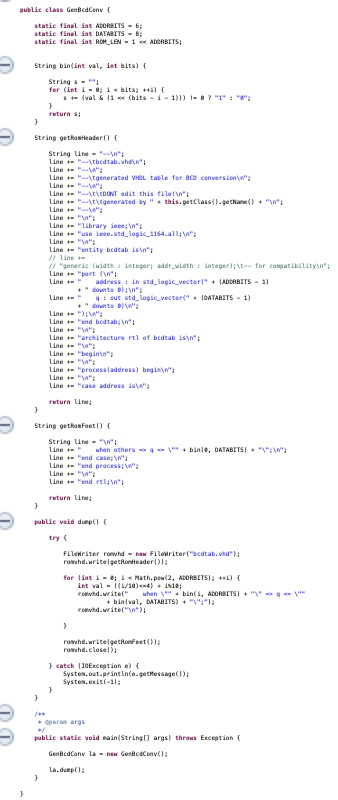
\includegraphics[scale=0.6]{JavaBCD}
\end{figure}
\end{frame}

\begin{frame}[fragile]{Java Program}
\begin{itemize}
\item Generates a VHDL table
\item The core code is:
\end{itemize}
\begin{chisel}
for (int i = 0; i < Math.pow(2, ADDRBITS); ++i) {
    int val = ((i/10)<<4) + i%10;
    // write out VHDL code for each line
\end{chisel}
\begin{itemize}
\item With all boilerplate 118 LoC
\end{itemize}
\end{frame}

\begin{frame}[fragile]{Chisel Version of Binary to BCD Conversion}
\begin{chisel}
  val array = new Array[Int](256)
  for (i <- 0 to 99) {
    array(i) = ((i/10)<<4) + i%10
  }
  val table = VecInit(array.map(_.U(8.W)))
\end{chisel}
\begin{itemize}
\item Directly generates the hardware (\code{VecInit})
\end{itemize}
\end{frame}

\begin{frame}[fragile]{Use Functional Programming for Generators}
\shortlist{../code/fun_first.txt}
\shortlist{../code/fun_func_lit.txt}
\shortlist{../code/fun_reduce_tree.txt}
\begin{itemize}
\item This is a simple example
\item What about an arbiter tree with fair arbitration?
\end{itemize}
\end{frame}

%\begin{frame}[fragile]{XXX}
%\begin{itemize}
%\item TODO: s4noc connection is part of the generator story
%\item
%\item
%\end{itemize}
%\end{frame}
%
%\begin{frame}[fragile]{XXX}
%\begin{itemize}
%\item
%\item
%\item
%\end{itemize}
%\end{frame}



\begin{frame}[fragile]{Generation Slides (inlude) are missing here}
\begin{itemize}
\item 
\end{itemize}
\end{frame}

\begin{frame}[fragile]{Combinational (Truth) Table Generation}
\begin{chisel}
val arr = new Array[Bits](length)
for (i <- 0 until length) {
  arr(i) = ...
}
val rom = Vec[Bits](arr)
\end{chisel}
\begin{itemize}
\item Generate a table in a Scala array
\item Use that array as input for a Chisel \code{Vec}
\item Generates a logic table at hardware construction time
\end{itemize}
\end{frame}

\begin{frame}[fragile]{Ideas for Runtime Table Generation}
\begin{itemize}
\item Assembler in Scala/Java generates the boot ROM
\item Table with a \code{sin} function
\item Binary to BCD conversion
\item Schedule table for a TDM based network-on-chip
\item 
\item More ideas?
\end{itemize}
\end{frame}

\begin{frame}[fragile]{Memory}
\begin{chisel}
val mem = Mem(Bits(width = 8), size)

// write
when(wrEna) {
  mem(wrAddr) := wrData
}

// read
val rdAddrReg = Reg(next = rdAddr)
rdData := mem(rdAddrReg)
\end{chisel}
\begin{itemize}
\item Write is synchronous
\item Read can be asynchronous or synchronous
\item But there are no asynchronous memories in an FPGA
\end{itemize}
\end{frame}

\begin{frame}[fragile]{Factory Methods}
\begin{itemize}
\item Simpler component creation and use
\item Usage similar to built in components, such as \code{Mux}
\end{itemize}
\begin{chisel}
val myAdder = Adder(x, y)
\end{chisel}
\begin{itemize}
\item A little bit more work on component side
\item Define an \code{apply} method on the companion object that returns the component
\end{itemize}
\begin{chisel}
object Adder {
  def apply(a: UInt, b: UInt) = {
    val adder = Module(new Adder)
    adder.io.a := a
    adder.io.b := b
    adder.io.result
  }
}
\end{chisel}
\end{frame}

\begin{frame}[fragile]{Summary}
\begin{itemize}
\item Chisel is a small language
\item Embedding it in Scala gives the power
\item We can write circuit generators
\item We can to co-simulation
\item We just scratched the surface
\end{itemize}
\end{frame}


\end{document}

\begin{frame}[fragile]{Summary}
\begin{itemize}
\item abc
\end{itemize}
\end{frame}
